\chapter{Obtaining the Equations of Motion using the Newton-Euler formulation and 
creating a preliminary Simulink model of the robotic arm}\label{chapter:1}
\vspace{-0.25cm}
Responsible: \textit{Sophie Sepp and Benedict Feldotto}

\section{Obtaining the Equations of Motion using the Newton-Euler formulation}
In chapter two a preliminary Simulink model of the robotic arm is created using the Newton Euler Formulation of the Equations of Motion. 



\subsection{Theoretical background}
To derive the equations of motion of the manipulator we use the Newton Euler Method. The equations of motion are used to compute the dynamic model of the robot. While in the Euler-Lagrange Equations the manipulator is treated as a whole and the analysis is performed using a Lagrangian function, in the Newton-Euler formulation each link of the robot is treated in turn.  Since each link is coupled to other links, the forces and torques of a link also appear in the equations describing its neighboring links. The whole process of deriving the terms of each link is called a forward-backward recursion.
In the forward phase we obtain the rotational velocities and accelerations using the following equations, where i+1 denotes the following link to the link i.


\begin{figure}[htsb]
  \centering
  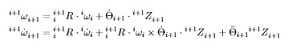
\includegraphics{figures/Rotational velocities and accelerations.jpg}
  \caption{Rotational velocities and accelerations.}
\end{figure}

\\For the linear accelerations of the single joints we use the formula:
\ \\
\begin{figure}
  \centering
  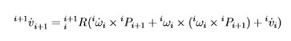
\includegraphics{figures/Linear accelerations of single joints.jpg}
  \caption{Linear accelerations of single joints.}
\end{figure}





\\To find the linear acceleration of the center of mass of each link we use:







\ \\
\begin{figure}[htsb]
  \centering
  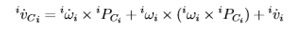
\includegraphics{figures/Linear acceleration for the center of mass of each link.jpg}
  \caption{Linear acceleration for the center of mass of each link.}
\end{figure}







\\In the backwards phase we use the following equations to compute the forces and torques at the center of mass of each link und the forces and torques acting on each joint:




\begin{figure}[htsb]
  \centering
  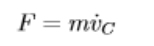
\includegraphics{figures/Equation Force.jpg}
  \caption{Equation Force.}
 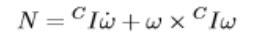
\includegraphics{figures/Equation Torque 1.jpg}
  \caption{Equation Torque 1.}
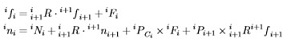
\includegraphics{figures/Forces and torques acting on each joint.jpg}
  \caption{Forces and torques acting on each joint.}
\end{figure}


  





\subsection{Implementing the equations in Matlab}
We first create a Simulink model of three links connected to the given initial constants and to the end effector. Each matlab function block holds a function to compute with the given input parameters the output parameters which become the input parameters of the next link. Thus all links are connected and compute the next values according to the input values they get from the previous link. This is done for the forward phase as well as for the backward phase. In the forward phase the linear and rotational velocities and accelerations of each link are computed. In the backwards phase the forces and torques that act on the centers of mass of each link are computed (Fi, Ni) and the forces and the torques that act on the single joints (fi, ni).



\begin{figure}[htsb]
  \centering
  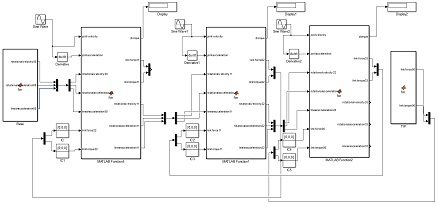
\includegraphics{figures/Three Links.jpg}
  \caption{Three Links.}
\end{figure}

\clearpage
\section{Implementing the Simulink Model}


